\documentclass[a4paper]{article} % {scrartcl} % for \subtitle
\usepackage[italian]{babel} 
\usepackage[utf8]{inputenc}
\usepackage[T1]{fontenc}
\usepackage{graphicx}
\usepackage{subfigure}
\usepackage{amsmath,amssymb, amsthm}
\usepackage{hyperref}
\hypersetup{
  colorlinks, linkcolor=blue
}
% \newcommand{\R}{\mathbb{R}}
% \newcommand{\N}{\mathbb{N}}

% \theoremstyle{plain}
% \newtheorem{teorema}{Teorema}

% \theoremstyle{plain}
% \newtheorem{proposizione}{Proposizione}

% \theoremstyle{definition}
% \newtheorem{definizione}{Definizione}

\author{Gianmarco Brocchi}
\title{Weighted Nonnegative Matrix Factorization \\
and Face Feature Extraction \\ - \\ un'implementazione}
% \subtitle{Un'implementazione}
\date{\today}

\begin{document}
\maketitle

Usando l'algoritmo suggerito nell'articolo di Vincent D. Blondel, Ngoc-Diep Ho e  Paul van Dooren si vuole applicare la WNMF ad una raccolta di immagini in modo da enfatizzare certe zone della matrice che le rappresenta. In particolare verranno usate immagini di volti.

\section{L'algoritmo}

\subsection{Kullback-Leibler Divergence}\label{KL-div}
Per studiare la convergenza del metodo vengono proposte regole di aggiornamento sotto le quali non aumentano, rispettivamente, la \emph{norma euclidea} e la \emph{Kullback-Leibler Divergence}; quest'ultima è una stima non simmetrica della differenza tra due distribuzioni di probabilità. Nello specifico, date due distribuzioni di probabilità $P$ e $Q$, la divergenza Kullback–Leibler di $Q$ da $P$, indicata con $D_{KL}(P \lVert Q)$, è una misura dell'informazione persa quando $Q$ è usata per approssimare $P$. Tale misura è spesso scelta nell'approssimazione di immagini come nel nostro caso.

Data la matrice $A$, la sua distanza dalla fattorizzazione $UV$ è:
\[ D(A \lVert UV) := \sum_{ij} \left[ A \circ \log_{\circ} \frac{[A]}{[UV]} - A + UV \right]_{ij} \]

Data la matrice $A$, stimeremo la sua distanza dalla fattorizzazione $UV$ con la \emph{KL-divergence} pesata con $W$ in questo modo:
\[ D_W(A \lVert UV) := \sum_{ij} \left[ W \circ \left( A \circ \log_{\circ} \frac{[A]}{[UV]} - A + UV \right) \right]_{ij} \]

\subsection{Update rules}
La divergenza pesata in \ref{KL-div} non aumenta con i seguenti aggiornamenti:

\[ \frac{[V]}{[U^tW]} \circ \left( U^t \frac{[W \circ A]}{[UV]} \right) \rightarrow V \text{ , } \frac{[U]}{[WV^t]} \circ \left( \frac{W \circ A}{[UV]}V^t \right) \rightarrow U \]

la divergenza $D_W(A\lVert UV)$ non cresce con tali aggiornamenti sse $U$ e $V$ sono non negative.

\subsection{Conversione}\label{subsec:conversione}
Le immagini, per poter applicare l'algoritmo, sono state convertite da formato RAW in ASCII e rinumerate da $1$ a $400$ per un più semplice recupero delle stesse. Per fare ciò è stato usata la libreria \texttt{PGMA TO PGMB} 
(in \texttt{C++}), rilasciata da John Burkardt sotto licenza libera (LGPL).
Vedi \ref{itm:A2B}.

\subsection{Librerie} 
Per leggere e scrivere i file PGM è stata utilizzata la libreria \texttt{PGMA IO} (per Fortran90), scritta da John Burkardt e rilasciata sotto licenza libera (LGPL).
Vedi \ref{itm:IO}.

\subsection{Makefile}
Per testare il progetto è possibile clonare il necessario via \texttt{git} all'indirizzo:\\
\begin{center} \url{http://poisson.phc.unipi.it/~brocchi/git/WNMF/} \end{center}

Dalla cartella è possibile dare i seguenti comandi:
\begin{description}
\item[\texttt{make}]: compilerà i sorgenti \texttt{Fortran90} e li linkerà nell'eseguibile \texttt{PGM}
\item[\texttt{make run}]: esegue un \texttt{make} e lancia in automatico l'eseguibile
\item[\texttt{make faces}]: si occupa di scaricare il database dei volti, scompattarlo, compilare il convertitore e convertire le immagini in \texttt{ASCII}, rinumerandole in ordine crescente nella cartella \texttt{faces}
\item[\texttt{make clean / cclean}]: elimina e pulisce file binari e temporanei
\item[\texttt{make whole}]: esegue sia un \texttt{make faces} che un \texttt{make}, insieme a \texttt{run} esegue direttamente il programma.
\end{description}

\section{I dati}
L'algoritmo lavora su dati ottenuti dall'\texttt{ORL} face database\footnote{un insieme di volti dall'Olivetti Research Laboratory di Cambridge, UK} - vedi \ref{itm:ORL}.
Nello specifico si tratta di $400$ volti ($10$ immagini di $40$ soggetti). Le immagini sono in formato PGM\footnote{Portable Gray Map format}, ovvero in scala di grigi; tali immagini possono essere in formato RAW o ASCII, nel primo i valori di grigio sono memorizzati come semplici byte, nel secondo sono rappresentati da numeri tra 0 e 255. \\ 
(Nota: le immagini dell'\texttt{ORL} erano nel primo formato, pertanto è stato necessario convertirle: vedi \ref{subsec:conversione})

\section{Test}
Al fine di ottenere la miglior velocità di convergenza (e quindi il minor valore della \emph{KL-divergence} dopo un numero fissato di passi) sono state testate diverse implementazioni dell'algoritmo. In particolare, come accennato in \ref{article}, le matrici $U$ e $V$ possono essere:
\begin{itemize}
\item generate entrambe in modo random
\item generata random una e calcolata l'altra
\end{itemize}
Si è anche provato a ricalcolare $V$ a intervalli regolari durante gli aggiornamenti per migliorare la convergenza.
Inoltre sono state testate le varianti aggiornando $U$ e $V$ separatamente (ovvero senza usare l'ultimo aggiornamento di $U$ per aggiornare $V$) e scambiando l'ordine di aggiornamento.

\newpage
\section{Esempi}
Alcuni esempi di immagini:
\begin{figure}
  \centering
  \subfigure[Senza pesi]
  {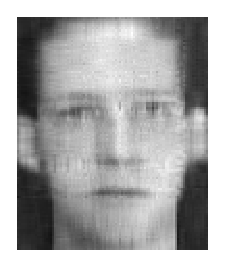
\includegraphics[scale=1.10]{img/singUV_noW_80.eps}}
  \subfigure[Con pesi centrati]
  {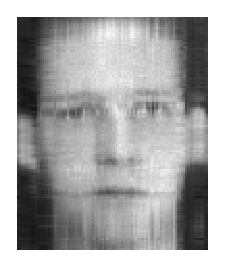
\includegraphics[scale=1.10]{img/singUV_80.eps}}
  \hspace{2mm}
  \subfigure[Originale]
  {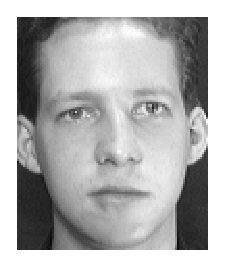
\includegraphics[scale=1.10]{img/original.eps}}
  \caption{Immagini dopo 80 iterazioni a confronto}
\end{figure}

\begin{figure}
  \centering
  \subfigure[Senza pesi]
  {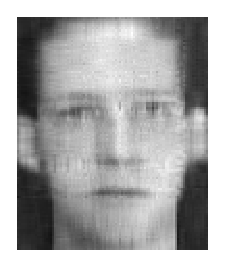
\includegraphics[trim = 5mm 20mm 5mm 12mm, clip=true, scale=1.60]{img/singUV_noW_80.eps}}
  \subfigure[Pesi centrati]
  {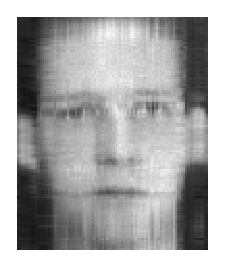
\includegraphics[trim = 5mm 20mm 5mm 12mm, clip=true, scale=1.60]{img/singUV_80.eps}}
  \subfigure[Originale]
  {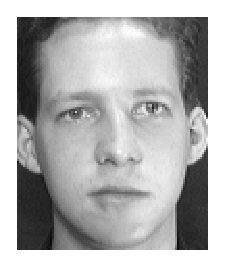
\includegraphics[trim = 5mm 20mm 5mm 12mm, clip=true, scale=1.60]{img/original.eps}}
  \caption{80 iterazioni, occhi a confronto}
\end{figure}

% \begin{figure}
%   \centering
%   \subfigure[Senza pesi]
%   {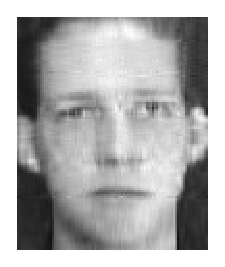
\includegraphics[scale=1.00]{img/singUV_noW_200.eps}}
%   \subfigure[Con pesi centrati]
%   {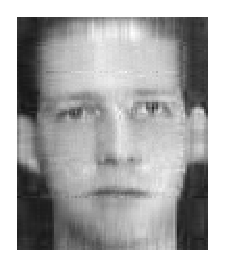
\includegraphics[scale=1.00]{img/singUV_200.eps}}
%   \hspace{2mm}
%   \subfigure[Originale]
%   {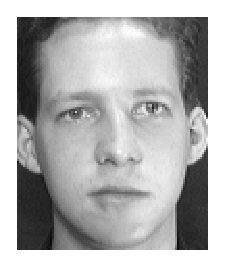
\includegraphics[scale=1.00]{img/original.eps}}
%   \caption{Immagini dopo 200 iterazioni a confronto}
% \end{figure}

\begin{figure}
  \centering
  \subfigure[Senza pesi]
  {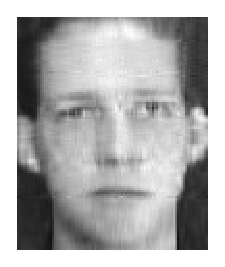
\includegraphics[trim = 5mm 20mm 5mm 12mm, clip=true, scale=1.70]{img/singUV_noW_200.eps}}
  \subfigure[Pesi centrati]
  {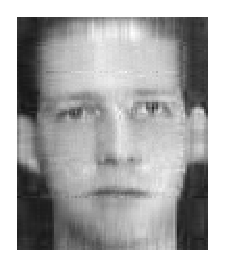
\includegraphics[trim = 5mm 20mm 5mm 12mm, clip=true, scale=1.70]{img/singUV_200.eps}}
  \subfigure[Originale]
  {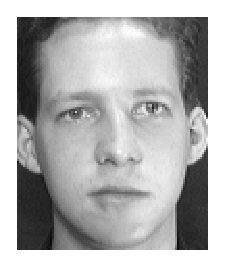
\includegraphics[trim = 5mm 20mm 5mm 12mm, clip=true, scale=1.70]{img/original.eps}}
  \caption{200 iterazioni, occhi a confronto}
\end{figure}

\newpage
\section{Link}
\begin{enumerate}
\item \texttt{ORL} face database \\
  \url{http://www.cl.cam.ac.uk/research/dtg/attarchive/facedatabase.html}\label{itm:ORL}

\item \texttt{PGMA TO PGMB} \\
  \url{http://people.sc.fsu.edu/~jburkardt/cpp_src/pgma_to_pgmb/pgma_to_pgmb.html}\label{itm:A2B}

\item \texttt{PGMA IO} \\
  \url{http://people.sc.fsu.edu/~jburkardt/f_src/pgma_io/pgma_io.html}\label{itm:IO}

\end{enumerate}

LIBNMF – A LIBRARY FOR NONNEGATIVE MATRIX FACTORIZATION, \\
A. Janecek, S. Schulze Grotthoff, W.N. Gansterer\label{article}

\end{document}

